\newcommand*{\addheight}[2][.5ex]{%
  \raisebox{0pt}[\dimexpr\height+(#1)\relax]{#2}%
}

\chapter{Experiments}\label{ch:Experiments} 
In this chapter, I will present the experiments conducted to test and verify the methods I
introduced. Furthermore, I will explain how to figure out what the best parameters for both corner detection and inpainting
are. Below, we can see all the test images that were used for the experiments.
\begin{figure}[h]
    \centering
    \fbox{
\includegraphics[width=0.2\linewidth]{../../images/binary/rect_tiny.png}}
    \fbox{
\includegraphics[width=0.2\linewidth]{../../images/binary/flatcorner.png}}
    \fbox{
\includegraphics[width=0.2\linewidth]{../../images/binary/corner.png}}\\\vspace{0.2cm}
    \fbox{
\includegraphics[width=0.2\linewidth]{../../images/binary/abstract1_small.png}}
    \fbox{
\includegraphics[width=0.2\linewidth]{../../images/binary/cat.png}}
    \fbox{
\includegraphics[width=0.2\linewidth]{../../images/binary/ellipse_small.png}}
    \caption{Binary test images. From top left to bottom right: \texttt{rect\_tiny},
    \texttt{flatcorner1}, \texttt{corner}, \texttt{abstract1\_small}, \texttt{cat},
\texttt{ellipse\_small}. Image \texttt{cat} provided by Joachim Weickert. Remaining images created
with GIMP}\label{fig:BinaryImages}
\end{figure}
\begin{figure}[h]
    \centering
    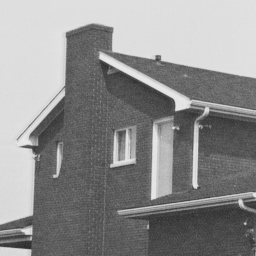
\includegraphics[width=0.3\linewidth]{../../images/grey/house.png}
    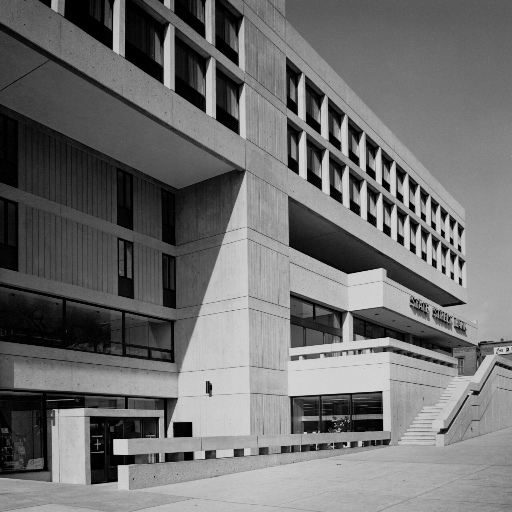
\includegraphics[width=0.3\linewidth]{../../images/grey/bank.png}
    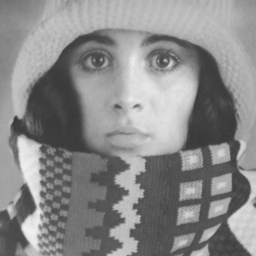
\includegraphics[width=0.3\linewidth]{../../images/grey/trui.png}
    \caption{(8-bit) Grayscale test images. From left to right: \texttt{house}, \texttt{bank},
    \texttt{trui}. Images provided by Joachim Weickert.}\label{fig:GreyImages}
\end{figure}
\section{Parameter Selection}\label{sec:ParameterSelection}
Both the corner detection process and the inpainting process introduce many parameters that need to
be chosen carefully to get the best results. The focus in this thesis lies mainly on examining the
choice of parameters for the corner localisation. While we will still explore how the parameters in
the reconstruction step influence the quality of the end result, it will interesting be to
see what role the mask radius plays in this context.

\subsection{Corner Detection}\label{sec:CornerEx}
In the corner detection phase, we differentiate between 4 parameters:
\begin{itemize}
    \item the noise scale $\sigma$
    \item the integration scale $\rho$
    \item the percentile parameter $p$ and
    \item the mask radius (also radius for circular non-maximum suppression) $R$
\end{itemize}
Depending on whether one chooses to use the circular non-maximum suppression (CNMS) and the total pixel
percentage thresholding (TPPT), the mask radius and percentile parameter will have different or additional
meaning.
The percentile parameter determines either the percentage of corners (without TPPT) to keep or the maximum bound
on the pixel density in the inpainting mask (with TPPT).
The mask radius also serves as the radius for the neighbourhood in the CNMS procedure.\\
Regarding the noise scale, we generally want to choose it as large as necessary but keep it as small as
possible, meaning that we want to choose the smallest noise scale that gets rid of most of the
noise in the image since with a larger $\sigma$ 
one often faces the problem that the detected corners can not be located as accurately anymore,
since more and more relevant features are smoothed away (see~\ref{sub:ScaleSpaces}). Another problem
is that the gaussian scale space (iterated gaussian smoothing) may even introduce new
corners~\cite{weickert96}.
 Most of the time however, a $\sigma$ of 1 is sufficient enough to remove most of the noise and unnecessary
 details and still provide an accurate result.\\
 The integration scale $\rho$ is an interesting parameter as it basically determines how well the
 corner can be localised. Here, one has to be careful as the choice of this parameter is somewhat
 dependent on the noise scale in the sense that the integration scale always should be 
 at least as large as the noise scale.\\
 On the other hand, by increasing the integration scale, we also increase the inaccuracy in the corner 
 localisation as we see in figure~\ref{fig:Integration}.
\begin{figure}[h]
    \centering
    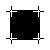
\includegraphics[width=0.4\linewidth]{rect/rect_2_corner.png}
    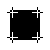
\includegraphics[width=0.4\linewidth]{rect/rect_4_corner.png}
    
\includegraphics[width=0.4\linewidth]{rect/rect_6_corner.png}
    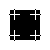
\includegraphics[width=0.4\linewidth]{rect/rect_8_corner.png}
    \caption{Location of corners with different values for $\rho$.\\
\textbf{Top left:} $\rho=2$, \textbf{Top right:} $\rho=4$, \textbf{Bottom left:}
$\rho=6$, \textbf{Bottom right} $\rho=8$. Original image: \texttt{rect\_tiny} (see Figure~\ref{fig:BinaryImages})}\label{fig:Integration}
\end{figure}
This demonstrates the issue mentioned in Chapter~\ref{ch:RelatedWork} with Zimmer's approach~\cite{zimmer07} quite nicely. 
We can see that with increasing integration scale, the inaccuracy increases
steadily. The problem with Zimmer's approach is that they did not adress these inaccuracies in
their mask generation. They fixed the mask radius to be just a small neighbourhood of 4 to 8 pixels.
To adjust the amount of corners introduced into the mask, they adapted the integration scale.
Obviously this introduces the aforementioned inaccuracies and combined with the fixed neighbourhood
size, can lead to the actual corner not even being included in the final mask (see figure
~\ref{fig:Inacc}).
\begin{figure}[h]
    \centering
    
\includegraphics[width=0.4\linewidth]{rect/rect_2_mask_position.png}
    
\includegraphics[width=0.4\linewidth]{rect/rect_4_mask_position.png}
    \caption{Position of corner regions for examples from Figure~\ref{fig:Integration}.
        Position of the corner in white. Size of the corner region: 9px (8-neighbourhood)
    \textbf{Left:} $\rho=2$, \textbf{Right:} $\rho=4$ (Corner regions in grey for visualisation
purposes, not the actual mask). Original image: \texttt{rect\_tiny} (see Figure~\ref{fig:BinaryImages})}\label{fig:Inacc}
\end{figure}
We will discuss the optimal choice for the mask radius in the next section (\ref{sec:MaskEx}), but
first I will show some examples demonstrating the ideas behind the methods introduced in
Section~\ref{sub:Percentile} and~\ref{sub:Suppression}. As we can see in
figure~\ref{fig:CNMSExample}, CNMS allows us to distribute the corner regions in the mask more
evenly across the whole image. \\\ \\
While in the example without CNMS, most of the corners are
overlapping and grouped up in the lower half of the image; using CNMS, the overlapping corners are
removed and free up slots for corners with a lower cornerness measure, i.e.\ less sharp corners in
the upper half. Later in Figure~\ref{fig:AbstractCNMSExamples}, we can also observe that thanks to
CNMS, a few extra slots are freed up to be used in other regions.
\begin{figure}
    \centering
    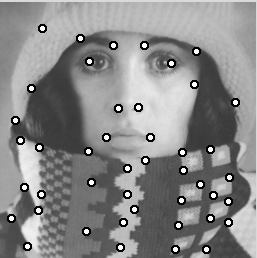
\includegraphics[width=0.31\linewidth]{trui/trui_corners_cnms.png}
    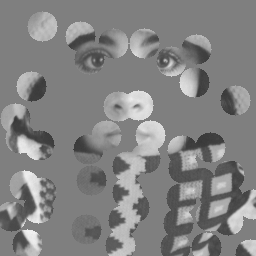
\includegraphics[width=0.31\linewidth]{trui/trui-mask_cnms.png}
    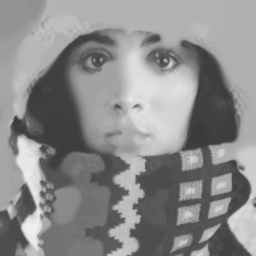
\includegraphics[width=0.31\linewidth]{trui/trui-inpaint_cnms.png}\\
    \vspace{0.2cm}
    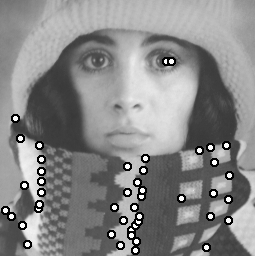
\includegraphics[width=0.31\linewidth]{trui/trui_corners_non_cnms.png}
    
\includegraphics[width=0.31\linewidth]{trui/trui-mask_non_cnms.png}
    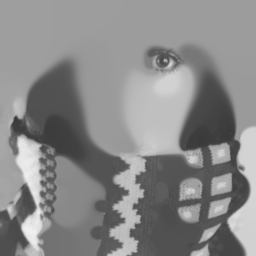
\includegraphics[width=0.31\linewidth]{trui/trui-inpaint_non_cnms.png}
    \caption{Effect of circular non maximum suppression on spread of corners across the image.
        \textbf{Top row:} Position of corners, inpainting mask and inpainting results
        \textbf{with} CNMS\@.
\textbf{Bottom row:} Position of corners, inpainting mask and inpainting results \textbf{without}
CNMS\@.
    Corner detection with Foerstner-Harris corner detector, $\sigma=1,\rho=2.5,R=15$ and a
percentile of 0.5. Original image: \texttt{trui} (see Figure~\ref{fig:GreyImages})}\label{fig:CNMSExample}
\end{figure}
\begin{figure}[h]
    \centering
    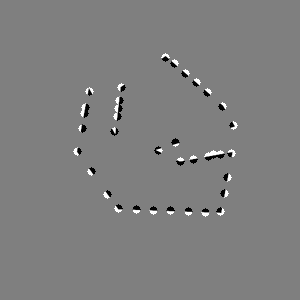
\includegraphics[width=0.4\linewidth]{abstract/abstract1_small-mask.png}\hspace{0.2cm}
    
\includegraphics[width=0.4\linewidth]{abstract/abstract1_small-inpaint.png}\\
    \vspace*{0.2cm}
    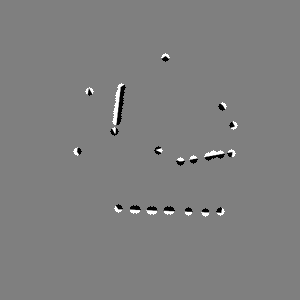
\includegraphics[width=0.4\linewidth]{abstract/abstract1_small-mask_no_cnms.png}\hspace{0.2cm}
    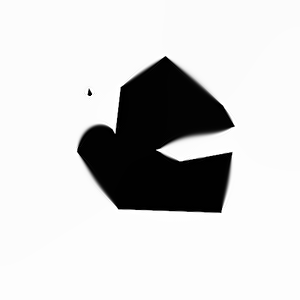
\includegraphics[width=0.4\linewidth]{abstract/abstract1_small-inpaint_no_cnms.png}\\
    \caption{Demonstration of the effects of CNMS on the spread of corner regions.
\textbf{Top row:} $\sigma=1,\rho=1,R=4,q=0.02$, with CNMS, Pixel density: 1.96\%, PSNR\@:
31.45
\textbf{Bottom row:} $\sigma=1,\rho=1,R=4,q=0.02$, without CNMS, Pixel density:
1.51\%, PSNR\@: 21.12
Inpainting parameters: $\sigma=2,\lambda=0.1,\alpha=0.49,\gamma=1,N=1000$
Original image: \texttt{abstract1\_small} (see Figure~\ref{fig:BinaryImages})}\label{fig:AbstractCNMSExamples}
\end{figure}
\begin{figure}[ht]
    \centering
    
\includegraphics[width=0.3\linewidth]{tppt_ex/abstract1_small4.png}
    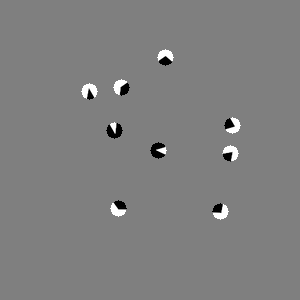
\includegraphics[width=0.3\linewidth]{tppt_ex/abstract1_small8.png}
    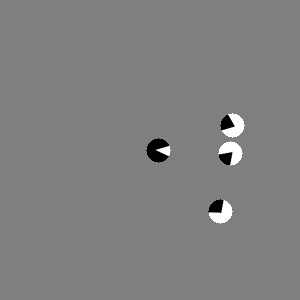
\includegraphics[width=0.3\linewidth]{tppt_ex/abstract1_small12.png}
    \caption{Effect of TPPT\@. Upper bound on the pixel density: 2\%. Actual values:
        1.95\%, 1.97\%, 1.96\%. Original image: \texttt{abstract1\_small} (see
    Figure~\ref{fig:BinaryImages})}\label{fig:TPPTEx}
\end{figure}
\\\noindent In Figure~\ref{fig:TPPTEx}, we can also see that TPPT actually produces masks of a
similar size, bound by the percentage given by the parameter $p$. What I also noticed is that the
percentage is not as accurate when using a normal non-maximum suppression approach. This is due to
the potential overlap that is not accounted for in the initial estimation of the amount of corner
regions that can be introduced into the mask.
However, the TPPT approach is not perfect.\\
It does not always yield accurate masks since for one
reason, the maximum possible pixel density depends on the amount of corners detected. On the other
hand, with increasing mask radius it is also harder to get an accurate pixel density. Some possible
remedies would include having variable mask radii, inserting random pixels as a post processing
step to fill up the
remaining percentage or, instead of using the parameter as an upper bound, simply minimising the
squared error (i.e.\ allow overshoots).
\newpage\noindent
\subsection{Inpainting}\label{sec:InpaintingEx}
As already mentioned, we are using an EED-based inpainting algorithm with a Charbonnier diffusivity
as explained in Section~\ref{sec:Inpainting}.
The main parameters required by the inpainting process are 
\begin{itemize}
    \item the noise scale $\sigma$,
    \item the integration scale $\rho$,
    \item the contrast parameter $\lambda$, 
    \item the dissipativity parameter $\alpha$ and
    \item a non-negativity parameter $\gamma$.
\end{itemize}
If we recall from Section~\ref{sec:Inpainting}, when using EED, we do not need the integation scale, as the
integration scale only influences the radius of the structure tensor which is actually not needed
for this method of inpainting. Thus, this parameter will be fixed to 0.\\
The parameters $\alpha$ and $\gamma$ are purely numerical parameters that are used to 
stabilise the algorithm or rather help to ensure that the stencil weights of the discretisation of
the diffusion process meet certain requirements.
In this work I fixed these parameters to $\alpha=0.49,\, \gamma=1.0$~\cite{conversation}.
In general, one could image the parameter $\alpha$ as a sharpness parameter: the larger the
$\alpha$ (but not larger than 0.5), the sharper the image. More on the nature of these two parameters can be read about in
~\cite{www13, weickert96}.\\
More interesting is the contrast parameter $\gamma$ that is required in the diffusivity function
\eqref{def:Diffusivity}. As already explained in Section~\ref{sec:Structure}, this parameter helps to
distinguish between edges and non-edges. For the EED inpainting this is especially important since
it basically determines how strongly edges will be continued into inpainting regions. \\
The caveat with this parameter is that even though a smaller $\lambda\ (\leq0.1)$ yields very sharp
results, especially for binary images, it increases the chance of the algorithm becoming unstable.
Normally a $\lambda<0.1$ should not be used~\cite{conversation}. Since the optimal choice for this parameter is still a
topic of current research, I had to experiment a little to find the best choice. Furthermore it was
suggested that the optimal $\lambda$ depends on the input image~\cite{schmaltz14}. 
The noise scale $\sigma$ was always chosen to be somewhere between 1 and 4 as this seemed to give
the best results.
\section{Mask Radius}\label{sec:MaskEx}
By introducing the mask radius as an additional parameter, we now have to pose the question of what
radius would yield the best result. One hypothesis is that it would be best to compute the the
mask radius in dependence of the integration scale $\rho$, in order to account for the inaccuracies
mentioned in Section~\ref{sec:CornerEx}~\cite{conversation}.
\begin{figure}[h]
    \centering
    
\includegraphics[width=0.2\linewidth]{disctest/flatcorner1.png}\hspace{0.2cm}
    
\includegraphics[width=0.2\linewidth]{disctest/flatcorner1mask.png}\hspace{0.2cm}
    
\includegraphics[width=0.2\linewidth]{disctest/flatcorner1inpaint.png}\\
    \vspace*{0.2cm}
    
\includegraphics[width=0.2\linewidth]{disctest/flatcorner2.png}\hspace{0.2cm}
    
\includegraphics[width=0.2\linewidth]{disctest/flatcorner2mask.png}\hspace{0.2cm}
    
\includegraphics[width=0.2\linewidth]{disctest/flatcorner2inpaint.png}\\
    \vspace*{0.2cm}
    
\includegraphics[width=0.2\linewidth]{disctest/flatcorner3.png}\hspace{0.2cm}
    
\includegraphics[width=0.2\linewidth]{disctest/flatcorner3mask.png}\hspace{0.2cm}
    
\includegraphics[width=0.2\linewidth]{disctest/flatcorner3inpaint.png}\\
    \vspace*{0.2cm}
    
\includegraphics[width=0.2\linewidth]{disctest/flatcorner4.png}\hspace{0.2cm}
    
\includegraphics[width=0.2\linewidth]{disctest/flatcorner4mask.png}\hspace{0.2cm}
    
\includegraphics[width=0.2\linewidth]{disctest/flatcorner4inpaint.png}\\
    \vspace*{0.2cm}
    
\includegraphics[width=0.2\linewidth]{disctest/flatcorner5.png}\hspace{0.2cm}
    
\includegraphics[width=0.2\linewidth]{disctest/flatcorner5mask.png}\hspace{0.2cm}
    
\includegraphics[width=0.2\linewidth]{disctest/flatcorner5inpaint.png}\\
    \caption{Experiment with identical mask radius $R=4$ and varying integration scale. $\rho$ from top to bottom:
    1, 2, 3, 4, 5. PSNR from top to bottom: 12.49, 12.49, 12.49, 11.31, 8.09. Original image:
\texttt{flatcorner} (see Figure~\ref{fig:BinaryImages})}\label{fig:MaskEx}
\end{figure}
\newpage\noindent The hypothesis was tested by switching out the Gaussian
convolution in the computation of the structure tensor in the corner detection process for a
regular convolution with a so called \textit{normalised pillbox kernel}, which is basically just
averaging inside a disk-shaped neighbourhood, to get a better representation of the uncertainty in
the corner localisation~\cite{conversation}. After that, it was tested whether it would be
sensible in terms of reconstruction quality to choose a mask radius equal to the radius of the
pillbox kernel~\cite{conversation}. 
In Figure~\ref{fig:MaskEx} we can see the motivation behind the
idea. There we can see how the actual corner slowly moves out of the corner region for increasing
$\rho$. I should note that the corner locations and thus the masks and inpainting results for
$\rho=1,2,3$ are the same. The interesting thing however is that the quality suddenly drops when we 
have 
\begin{equation}
    \frac{R}{\rho}\leq1
\end{equation}
This observation motivated the next experiment in which I tested different integration scales
paired with multiple mask radii to create the matrix we can see in Figure~\ref{fig:InaccTestMask}.
Looking at the resulting inpainted images (see Figure~\ref{fig:InaccTestInpaint}) and their
respective PSNR values (see Figure~\ref{fig:InaccTestPSNR}), we observe a similar effect, namely
that the PSNR jumps by a large margin every time the ratio between the mask radius and the
integration scale goes beyond 1.
Another interesting observation is that the biggest jump is almost
always at a transition from a ratio smaller than 1 to a ratio of 1 (cells in grey), suggesting that
as soon as the inaccuracy is matched by the mask radius, the inpainting quality increases. The only
exception here is $\rho=3$. A possible explanation is that in this case, the corner
location is the same for both $\rho=2$ and $\rho=3$, which is why all the inpainted images and
masks are identical. Similar results can be observed in
Figure~\ref{fig:RectInaccTestPSNR}.\\
All in all we can say that the experiments provided reasonable proof that the hypothesis stated
above is true. As a corollary from this we can deduce that a more accurate corner detection method
could result in smaller mask sizes and ultimately better compression rates.
\begin{figure}[H]
    \centering
    \begin{tabular}{|c|cccccc|}
        \hline
        \diagbox{$\rho$}{$R$}&1&2&3&4&5&6\\\hline
        \raisebox{0.8cm}{1} &
        \addheight{
\includegraphics[width=0.12\linewidth]{inacctest/cornerr1m1mask.png}}
          &
        \addheight{
\includegraphics[width=0.12\linewidth]{inacctest/cornerr1m2mask.png}}
          &
        \addheight{
\includegraphics[width=0.12\linewidth]{inacctest/cornerr1m3mask.png}}
          &
        \addheight{
\includegraphics[width=0.12\linewidth]{inacctest/cornerr1m4mask.png}}
          &
        \addheight{
\includegraphics[width=0.12\linewidth]{inacctest/cornerr1m5mask.png}}
          &
        \addheight{
\includegraphics[width=0.12\linewidth]{inacctest/cornerr1m6mask.png}}\\
        \raisebox{0.8cm}{2} &
        \addheight{
\includegraphics[width=0.12\linewidth]{inacctest/cornerr2m1mask.png}}
          &
        \addheight{\includegraphics[width=0.12\linewidth]{inacctest/cornerr2m2mask.png}}
          &
        \addheight{\includegraphics[width=0.12\linewidth]{inacctest/cornerr2m3mask.png}}
          &
        \addheight{\includegraphics[width=0.12\linewidth]{inacctest/cornerr2m4mask.png}}
          &
        \addheight{\includegraphics[width=0.12\linewidth]{inacctest/cornerr2m5mask.png}}
          &
        \addheight{\includegraphics[width=0.12\linewidth]{inacctest/cornerr2m6mask.png}}\\
        \raisebox{0.8cm}{3} &
        \addheight{\includegraphics[width=0.12\linewidth]{inacctest/cornerr3m1mask.png}}
          &
        \addheight{\includegraphics[width=0.12\linewidth]{inacctest/cornerr3m2mask.png}}
          &
        \addheight{\includegraphics[width=0.12\linewidth]{inacctest/cornerr3m3mask.png}}
          &
        \addheight{\includegraphics[width=0.12\linewidth]{inacctest/cornerr3m4mask.png}}
          &
        \addheight{\includegraphics[width=0.12\linewidth]{inacctest/cornerr3m5mask.png}}
          &
        \addheight{\includegraphics[width=0.12\linewidth]{inacctest/cornerr3m6mask.png}}\\
        \raisebox{0.8cm}{4} &
        \addheight{\includegraphics[width=0.12\linewidth]{inacctest/cornerr4m1mask.png}}
          &
        \addheight{\includegraphics[width=0.12\linewidth]{inacctest/cornerr4m2mask.png}}
          &
        \addheight{\includegraphics[width=0.12\linewidth]{inacctest/cornerr4m3mask.png}}
          &
        \addheight{\includegraphics[width=0.12\linewidth]{inacctest/cornerr4m4mask.png}}
          &
        \addheight{\includegraphics[width=0.12\linewidth]{inacctest/cornerr4m5mask.png}}
          &
        \addheight{\includegraphics[width=0.12\linewidth]{inacctest/cornerr4m6mask.png}}\\
        \raisebox{0.8cm}{5} &
        \addheight{\includegraphics[width=0.12\linewidth]{inacctest/cornerr5m1mask.png}}
          &
        \addheight{\includegraphics[width=0.12\linewidth]{inacctest/cornerr5m2mask.png}}
          &
        \addheight{\includegraphics[width=0.12\linewidth]{inacctest/cornerr5m3mask.png}}
          &
        \addheight{\includegraphics[width=0.12\linewidth]{inacctest/cornerr5m4mask.png}}
          &
        \addheight{\includegraphics[width=0.12\linewidth]{inacctest/cornerr5m5mask.png}}
          &
        \addheight{\includegraphics[width=0.12\linewidth]{inacctest/cornerr5m6mask.png}}\\\hline
    \end{tabular}
    \caption{Inpainting masks for image corner.pgm for varying integration scale and mask radius.
    Original image: \texttt{corner} (see Figure~\ref{fig:BinaryImages})}\label{fig:InaccTestMask}
\end{figure}
\begin{figure}[H]
    \centering
    \begin{tabular}{|c|cccccc|}
        \hline
        \diagbox{$\rho$}{$R$}&1&2&3&4&5&6\\\hline
        \raisebox{0.8cm}{1} &
        \addheight{\includegraphics[width=0.12\linewidth]{inacctest/cornerr1m1inpaint.png}}
          &
        \addheight{\includegraphics[width=0.12\linewidth]{inacctest/cornerr1m2inpaint.png}}
          &
        \addheight{\includegraphics[width=0.12\linewidth]{inacctest/cornerr1m3inpaint.png}}
          &
        \addheight{\includegraphics[width=0.12\linewidth]{inacctest/cornerr1m4inpaint.png}}
          &
        \addheight{\includegraphics[width=0.12\linewidth]{inacctest/cornerr1m5inpaint.png}}
          &
        \addheight{\includegraphics[width=0.12\linewidth]{inacctest/cornerr1m6inpaint.png}}\\
        \raisebox{0.8cm}{2} &
        \addheight{\includegraphics[width=0.12\linewidth]{inacctest/cornerr2m1inpaint.png}}
          &
        \addheight{\includegraphics[width=0.12\linewidth]{inacctest/cornerr2m2inpaint.png}}
          &
        \addheight{\includegraphics[width=0.12\linewidth]{inacctest/cornerr2m3inpaint.png}}
          &
        \addheight{\includegraphics[width=0.12\linewidth]{inacctest/cornerr2m4inpaint.png}}
          &
        \addheight{\includegraphics[width=0.12\linewidth]{inacctest/cornerr2m5inpaint.png}}
          &
        \addheight{\includegraphics[width=0.12\linewidth]{inacctest/cornerr2m6inpaint.png}}\\
        \raisebox{0.8cm}{3} &
        \addheight{\includegraphics[width=0.12\linewidth]{inacctest/cornerr3m1inpaint.png}}
          &
        \addheight{\includegraphics[width=0.12\linewidth]{inacctest/cornerr3m2inpaint.png}}
          &
        \addheight{\includegraphics[width=0.12\linewidth]{inacctest/cornerr3m3inpaint.png}}
          &
        \addheight{\includegraphics[width=0.12\linewidth]{inacctest/cornerr3m4inpaint.png}}
          &
        \addheight{\includegraphics[width=0.12\linewidth]{inacctest/cornerr3m5inpaint.png}}
          &
        \addheight{\includegraphics[width=0.12\linewidth]{inacctest/cornerr3m6inpaint.png}}\\
        \raisebox{0.8cm}{4} &
        \addheight{\includegraphics[width=0.12\linewidth]{inacctest/cornerr4m1inpaint.png}}
          &
        \addheight{\includegraphics[width=0.12\linewidth]{inacctest/cornerr4m2inpaint.png}}
          &
        \addheight{\includegraphics[width=0.12\linewidth]{inacctest/cornerr4m3inpaint.png}}
          &
        \addheight{\includegraphics[width=0.12\linewidth]{inacctest/cornerr4m4inpaint.png}}
          &
        \addheight{\includegraphics[width=0.12\linewidth]{inacctest/cornerr4m5inpaint.png}}
          &
        \addheight{\includegraphics[width=0.12\linewidth]{inacctest/cornerr4m6inpaint.png}}\\
        \raisebox{0.8cm}{5} &
        \addheight{\includegraphics[width=0.12\linewidth]{inacctest/cornerr5m1inpaint.png}}
          &
        \addheight{\includegraphics[width=0.12\linewidth]{inacctest/cornerr5m2inpaint.png}}
          &
        \addheight{\includegraphics[width=0.12\linewidth]{inacctest/cornerr5m3inpaint.png}}
          &
        \addheight{\includegraphics[width=0.12\linewidth]{inacctest/cornerr5m4inpaint.png}}
          &
        \addheight{\includegraphics[width=0.12\linewidth]{inacctest/cornerr5m5inpaint.png}}
          &
        \addheight{\includegraphics[width=0.12\linewidth]{inacctest/cornerr5m6inpaint.png}}\\\hline
    \end{tabular}
    \caption{Inpainting results for mask shown in Figure~\ref{fig:InaccTestMask}. Inpainting
    parameters: $\sigma=2,\lambda=0.4,\alpha=0.49,\gamma=1$. Original image: \texttt{corner} (see Figure~\ref{fig:BinaryImages})}\label{fig:InaccTestInpaint}
\end{figure}
\begin{figure}[H]
    \centering
    \begin{tabular}{|c|c|c|c|c|c|c|}
        \hline
        \diagbox{$\rho$}{$R$}&1&2&3&4&5&6\\\hline
        1 & \cellcolor{gray!25}\textbf{4.83} & \textbf{10.97} & 15.70 & 20.39 & 22.71 & 23.58 \\\hline
        2 & 1.25 & \cellcolor{gray!25}7.89 & \textbf{17.31} & \textbf{21.48} & \textbf{23.45} &
        24.13 \\\hline
        3 & 1.25 & 7.89 & \cellcolor{gray!25}\textbf{17.31} & \textbf{21.48} & \textbf{23.45} &
        24.13 \\\hline
        4 & 1.25 & 1.25 & 7.21 & \cellcolor{gray!25}16.91 & 22.92 & \textbf{24.34} \\\hline
        5 & 1.25 & 1.25 & 1.25 & 7.84 & \cellcolor{gray!25}17.96 & 22.82 \\\hline
    \end{tabular}
    \caption{PSNR values of the reconstructed images in
    Figure~\ref{fig:InaccTestInpaint}. Bold values are the best in the respective column.
Gray cells are cells where the $R$ and $\rho$ are equal.}\label{fig:InaccTestPSNR}
\end{figure}
\begin{figure}[H]
    \centering
    \begin{tabular}{|c|cccccc|}
        \hline
        \diagbox{$\rho$}{$R$}&1&2&3&4&5&6\\\hline
        \raisebox{0.8cm}{1} &
        \addheight{\includegraphics[width=0.12\linewidth]{rect_inacc/rect_tinyr1m1mask.png}}
          &
        \addheight{\includegraphics[width=0.12\linewidth]{rect_inacc/rect_tinyr1m2mask.png}}
          &
        \addheight{\includegraphics[width=0.12\linewidth]{rect_inacc/rect_tinyr1m3mask.png}}
          &
        \addheight{\includegraphics[width=0.12\linewidth]{rect_inacc/rect_tinyr1m4mask.png}}
          &
        \addheight{\includegraphics[width=0.12\linewidth]{rect_inacc/rect_tinyr1m5mask.png}}
          &
        \addheight{\includegraphics[width=0.12\linewidth]{rect_inacc/rect_tinyr1m6mask.png}}\\
        \raisebox{0.8cm}{2} &
        \addheight{\includegraphics[width=0.12\linewidth]{rect_inacc/rect_tinyr2m1mask.png}}
          &
        \addheight{\includegraphics[width=0.12\linewidth]{rect_inacc/rect_tinyr2m2mask.png}}
          &
        \addheight{\includegraphics[width=0.12\linewidth]{rect_inacc/rect_tinyr2m3mask.png}}
          &
        \addheight{\includegraphics[width=0.12\linewidth]{rect_inacc/rect_tinyr2m4mask.png}}
          &
        \addheight{\includegraphics[width=0.12\linewidth]{rect_inacc/rect_tinyr2m5mask.png}}
          &
        \addheight{\includegraphics[width=0.12\linewidth]{rect_inacc/rect_tinyr2m6mask.png}}\\
        \raisebox{0.8cm}{3} &
        \addheight{\includegraphics[width=0.12\linewidth]{rect_inacc/rect_tinyr3m1mask.png}}
          &
        \addheight{\includegraphics[width=0.12\linewidth]{rect_inacc/rect_tinyr3m2mask.png}}
          &
        \addheight{\includegraphics[width=0.12\linewidth]{rect_inacc/rect_tinyr3m3mask.png}}
          &
        \addheight{\includegraphics[width=0.12\linewidth]{rect_inacc/rect_tinyr3m4mask.png}}
          &
        \addheight{\includegraphics[width=0.12\linewidth]{rect_inacc/rect_tinyr3m5mask.png}}
          &
        \addheight{\includegraphics[width=0.12\linewidth]{rect_inacc/rect_tinyr3m6mask.png}}\\
        \raisebox{0.8cm}{4} &
        \addheight{\includegraphics[width=0.12\linewidth]{rect_inacc/rect_tinyr4m1mask.png}}
          &
        \addheight{\includegraphics[width=0.12\linewidth]{rect_inacc/rect_tinyr4m2mask.png}}
          &
        \addheight{\includegraphics[width=0.12\linewidth]{rect_inacc/rect_tinyr4m3mask.png}}
          &
        \addheight{\includegraphics[width=0.12\linewidth]{rect_inacc/rect_tinyr4m4mask.png}}
          &
        \addheight{\includegraphics[width=0.12\linewidth]{rect_inacc/rect_tinyr4m5mask.png}}
          &
        \addheight{\includegraphics[width=0.12\linewidth]{rect_inacc/rect_tinyr4m6mask.png}}\\
        \raisebox{0.8cm}{5} &
        \addheight{\includegraphics[width=0.12\linewidth]{rect_inacc/rect_tinyr5m1mask.png}}
          &
        \addheight{\includegraphics[width=0.12\linewidth]{rect_inacc/rect_tinyr5m2mask.png}}
          &
        \addheight{\includegraphics[width=0.12\linewidth]{rect_inacc/rect_tinyr5m3mask.png}}
          &
        \addheight{\includegraphics[width=0.12\linewidth]{rect_inacc/rect_tinyr5m4mask.png}}
          &
        \addheight{\includegraphics[width=0.12\linewidth]{rect_inacc/rect_tinyr5m5mask.png}}
          &
        \addheight{\includegraphics[width=0.12\linewidth]{rect_inacc/rect_tinyr5m6mask.png}}\\\hline
    \end{tabular}
    \caption{Inpainting masks for for varying integration scale and mask radius. Original image:
    \texttt{rect\_tiny} (see Figure~\ref{fig:BinaryImages})}\label{fig:RectInaccTestMask}
\end{figure}
\begin{figure}[H]
    \centering
    \begin{tabular}{|c|cccccc|}
        \hline
        \diagbox{$\rho$}{$R$}&1&2&3&4&5&6\\\hline
        \raisebox{0.8cm}{1} &
        \addheight{\includegraphics[width=0.12\linewidth]{rect_inacc/rect_tinyr1m1inpaint.png}}
          &
        \addheight{\includegraphics[width=0.12\linewidth]{rect_inacc/rect_tinyr1m2inpaint.png}}
          &
        \addheight{\includegraphics[width=0.12\linewidth]{rect_inacc/rect_tinyr1m3inpaint.png}}
          &
        \addheight{\includegraphics[width=0.12\linewidth]{rect_inacc/rect_tinyr1m4inpaint.png}}
          &
        \addheight{\includegraphics[width=0.12\linewidth]{rect_inacc/rect_tinyr1m5inpaint.png}}
          &
        \addheight{\includegraphics[width=0.12\linewidth]{rect_inacc/rect_tinyr1m6inpaint.png}}\\
        \raisebox{0.8cm}{2} &
        \addheight{\includegraphics[width=0.12\linewidth]{rect_inacc/rect_tinyr2m1inpaint.png}}
          &
        \addheight{\includegraphics[width=0.12\linewidth]{rect_inacc/rect_tinyr2m2inpaint.png}}
          &
        \addheight{\includegraphics[width=0.12\linewidth]{rect_inacc/rect_tinyr2m3inpaint.png}}
          &
        \addheight{\includegraphics[width=0.12\linewidth]{rect_inacc/rect_tinyr2m4inpaint.png}}
          &
        \addheight{\includegraphics[width=0.12\linewidth]{rect_inacc/rect_tinyr2m5inpaint.png}}
          &
        \addheight{\includegraphics[width=0.12\linewidth]{rect_inacc/rect_tinyr2m6inpaint.png}}\\
        \raisebox{0.8cm}{3} &
        \addheight{\includegraphics[width=0.12\linewidth]{rect_inacc/rect_tinyr3m1inpaint.png}}
          &
        \addheight{\includegraphics[width=0.12\linewidth]{rect_inacc/rect_tinyr3m2inpaint.png}}
          &
        \addheight{\includegraphics[width=0.12\linewidth]{rect_inacc/rect_tinyr3m3inpaint.png}}
          &
        \addheight{\includegraphics[width=0.12\linewidth]{rect_inacc/rect_tinyr3m4inpaint.png}}
          &
        \addheight{\includegraphics[width=0.12\linewidth]{rect_inacc/rect_tinyr3m5inpaint.png}}
          &
        \addheight{\includegraphics[width=0.12\linewidth]{rect_inacc/rect_tinyr3m6inpaint.png}}\\
        \raisebox{0.8cm}{4} &
        \addheight{\includegraphics[width=0.12\linewidth]{rect_inacc/rect_tinyr4m1inpaint.png}}
          &
        \addheight{\includegraphics[width=0.12\linewidth]{rect_inacc/rect_tinyr4m2inpaint.png}}
          &
        \addheight{\includegraphics[width=0.12\linewidth]{rect_inacc/rect_tinyr4m3inpaint.png}}
          &
        \addheight{\includegraphics[width=0.12\linewidth]{rect_inacc/rect_tinyr4m4inpaint.png}}
          &
        \addheight{\includegraphics[width=0.12\linewidth]{rect_inacc/rect_tinyr4m5inpaint.png}}
          &
        \addheight{\includegraphics[width=0.12\linewidth]{rect_inacc/rect_tinyr4m6inpaint.png}}\\
        \raisebox{0.8cm}{5} &
        \addheight{\includegraphics[width=0.12\linewidth]{rect_inacc/rect_tinyr5m1inpaint.png}}
          &
        \addheight{\includegraphics[width=0.12\linewidth]{rect_inacc/rect_tinyr5m2inpaint.png}}
          &
        \addheight{\includegraphics[width=0.12\linewidth]{rect_inacc/rect_tinyr5m3inpaint.png}}
          &
        \addheight{\includegraphics[width=0.12\linewidth]{rect_inacc/rect_tinyr5m4inpaint.png}}
          &
        \addheight{\includegraphics[width=0.12\linewidth]{rect_inacc/rect_tinyr5m5inpaint.png}}
          &
        \addheight{\includegraphics[width=0.12\linewidth]{rect_inacc/rect_tinyr5m6inpaint.png}}\\\hline
    \end{tabular}
    \caption{Inpainting results for mask shown in Figure~\ref{fig:RectInaccTestMask}. Inpainting
    parameters: $\sigma=2,\lambda=0.4,\alpha=0.49,\gamma=1$. Original image:
    \texttt{rect\_tiny} (see Figure~\ref{fig:BinaryImages})}\label{fig:RectInaccTestInpaint}
\end{figure}
\begin{figure}[H]
    \centering
    \begin{tabular}{|c|c|c|c|c|c|c|}
            \hline
            \diagbox{$\rho$}{$R$}&1&2&3&4&5&6\\\hline
            1 & \cellcolor{gray!25}\textbf{4.76} & 6.26 & 7.22 & 19.83 & 23.08 & 24.64 \\\hline
            2 & 1.93 & \cellcolor{gray!25}\textbf{9.71} & \textbf{19.41} & \textbf{22.86} & 24.54 & 25.63 \\\hline
            3 & 1.93 & \textbf{9.71} & \cellcolor{gray!25}\textbf{19.41} & \textbf{22.86} & 24.54 & 25.63 \\\hline
            4 & 1.93 & 1.93 & 9.51 & \cellcolor{gray!25}21.29 & \textbf{25.35} & 26.59 \\\hline
            5 & 1.93 & 1.93 & 1.93 & 14.39 & \cellcolor{gray!25}24.03 & \textbf{26.81} \\\hline
    \end{tabular}
    \caption{PSNR values of the reconstructed images in
        Figure~\ref{fig:RectInaccTestInpaint}. Bold values are the best in the respective column.
Gray cells are cells where the $R$ and $\rho$ are equal.}\label{fig:RectInaccTestPSNR}
\end{figure}
\newpage
\section{Examples}\label{sec:Results}
Finally, I will present some results of the reconstruction process using only corner regions as
seed points.
First up, I want to demonstrate the approach with multiple binary images shown in
Figure~\ref{fig:BinaryImages}. As we can see in Figure~\ref{fig:AbstractInpainting}, Figure~\ref{fig:RectInaccTestInpaint} and Figure~\ref{fig:InaccTestInpaint}, the algorithm works fairly well especially for binary
images with clearly defined corners even though the edges are not as sharp as one might have
hoped. However, the inpainting parameters were not highly optimised in these examples. The purpose
of these experiments was to show the influence of the ratio between mask radius and integration
scale on the final result. As a more practical example we see in Figure~\ref{fig:CatExample} that
piecewise straight edges can be reconstructed fairly well, whereas longer curves can be a challenge
for the algorithm.  On the other hand, curves pose a problem: the algorithm can
not really detect any corners there because of the small curvature (see Figure~\ref{fig:CatExample}). 
Thus, we have too little information to reconstruct this area properly. 
Finally, we can see that the method still works well, even with a bit of 
noise applied to it (see Figure~\ref{fig:AbstractNoise1})
However, if one increases the noise level we obsere that the quality of the reconstruction
deteriorates further, which is to be expected.
\begin{figure}[ht]
    \centering
    \vspace*{0.2cm}
    \includegraphics[width=0.4\linewidth]{abstract/abstract1_small-mask_larger_radius.png}\hspace{0.2cm}
    \includegraphics[width=0.4\linewidth]{abstract/abstract1_small-inpaint_larger_radius.png}
    \caption{Inpainting of image \texttt{abstract1\_small}. $\sigma=1,\rho=1,R=7,q=0.02$, Pixel
        density: 1.99\%, PSNR\@: 24.57, Inpainting parameters:
        $\sigma=2,\lambda=0.1,\alpha=0.49,\gamma=1,N=1000$, Original image:
        \texttt{abstract1\_small} (see Figure~\ref{fig:BinaryImages})}\label{fig:AbstractInpainting}
\end{figure}
\begin{figure}[ht]
    \centering
    \includegraphics[width=0.29\linewidth]{../../images/binary/abstract1_less_noise.png}
    \includegraphics[width=0.29\linewidth]{abstract/abstract1_less_noise-mask.png}
    \includegraphics[width=0.29\linewidth]{abstract/abstract1_less_noise-inpaint.png}
    \caption{Example of inpainting with noise degradation. Corner detection parameters:
    $\sigma=1.5,\rho=2.0,R=6,q=0.02$, Pixel density: 1.88\%, Inpainting parameters:
    $\sigma=2,\lambda=0.2,\alpha=0.49,\gamma=1$, PSNR\@: 20.74. Original image (without noise):
        \texttt{abstract1\_small} (see Figure~\ref{fig:BinaryImages})}\label{fig:AbstractNoise1}
\end{figure}
\begin{figure}[ht]
    \centering
    \includegraphics[width=0.29\linewidth]{../../images/binary/abstract1_noise.png}
    \includegraphics[width=0.29\linewidth]{abstract/abstract1_noise-mask.png}
    \includegraphics[width=0.29\linewidth]{abstract/abstract1_noise-inpaint.png}
    \caption{Example of inpainting with noise degradation. Corner detection parameters:
    $\sigma=1.5,\rho=2.0,R=6,q=0.02$, Pixel density: 1.88\%, Inpainting parameters:
$\sigma=2,\lambda=0.2,\alpha=0.49,\gamma=1$, PSNR\@: 16.25. Original image (without noise):
        \texttt{abstract1\_small} (see Figure~\ref{fig:BinaryImages})}\label{fig:AbstractNoise2}
\end{figure}                                       
\\ \noindent If we now look to more textured 8-bit grey value images like \texttt{house} and
\texttt{bank} (see Figure~\ref{fig:GreyImages}), we
see that the inpainting results become a bit worse compared to the binary images. This is primarily
due to the lacking availability of corners in natural images.\\\ \\
In Figure~\ref{fig:HouseEx}, we see that reconstruction using only the corners one would naturally
classify as corners (bottom row) is worse than the reconstruction where we added some corners that
would not qualify as a corner directly. For example the addition of the single corner region in the
top right corner improves the reconstruction in this area by a large margin, despite being more of
a part of an edge.
This same figure is also a prime example for the removal of textures if the textured regions are
underrepresented.
\begin{figure}[htpb]
    \centering
    \includegraphics[width=0.4\linewidth]{bank/bankr2m4mask.png}
    \includegraphics[width=0.4\linewidth]{bank/bankr2m4inpaint.png}\\\vspace{0.2cm}
    \caption{Inpaining of \texttt{bank}. Corner detection parameters:
        $\sigma=1,\rho=2,R=4,q=0.11$,TPPT+CNMS,
    Pixel density: 10.76\%, Inpainting parameters: $\sigma=2,\lambda=0.5,\alpha=0.49,\gamma=1$\\
PSNR:\@18.37. Original image: \texttt{bank} (see Figure~\ref{fig:GreyImages})}\label{fig:BankEx}
\end{figure}
\begin{figure}[h]
    \centering
    \includegraphics[width=0.4\linewidth]{cat/cat-mask1510.png}\hspace{0.2cm}
    \includegraphics[width=0.4\linewidth]{cat/cat-inpaint1510.png}
    \caption{Mask and inpainted result for cat.pgm. Corner detection parameters:
    $\sigma=1,\rho=1,R=10$, pixel density: 4.74\%, Inpainting parameters: $\sigma=2,\lambda=0.2$,
PSNR:\@18.35. Original image: \texttt{cat} (see Figure~\ref{fig:BinaryImages})}\label{fig:CatExample}
\end{figure}
\begin{figure}[h]
    \centering
    \includegraphics[width=0.2\linewidth]{ellipse_small-mask.png}
    \includegraphics[width=0.2\linewidth]{ellipse_small-inpaint.png}
    \caption{Example for the image ellipse\_small (see Figure~\ref{fig:BinaryImages}). Corner
    detection parameters: $\sigma=1,\rho=,R=4$. Inpainting parameters:
$\sigma=2,\lambda=0.1,\alpha=0.49,\gamma=1$. PSNR\@: 26.64. Original image: \texttt{ellipse} (see
Figure~\ref{fig:BinaryImages})}\label{fig:EllipseSmallExample}
\end{figure}
\begin{figure}[ht]
    \centering
    \includegraphics[width=0.4\linewidth]{house/house-mask.png}
    \includegraphics[width=0.4\linewidth]{house/house-inpaint.png}\\\vspace*{0.2cm}
    \includegraphics[width=0.4\linewidth]{house/house-mask3.png}
    \includegraphics[width=0.4\linewidth]{house/house-inpaint3.png}
    \caption{Mask and inpainting results of the image \texttt{house}. 
        \textbf{Top row: }Corner detection parameters: $\sigma=1,\rho=1,R=5,q=0.1, \text{CNMS}$, Pixel density: 9.23\%, Inpainting parameters:
    $\sigma=3,\lambda=0.2,\alpha=0.49,\gamma=1$, PSNR\@: 21.11\\
    \textbf{Bottom row: }Corner detection parameters: $\sigma=1,\rho=1.5,R=5,q=0.1, \text{no
    CNMS}$, Pixel density: 7.71\%, Inpainting parameters:
$\sigma=2,\lambda=0.4,\alpha=0.49,\gamma=1$, PSNR\@: 18.68. Original image: \texttt{house} (see
Figure~\ref{fig:GreyImages})}\label{fig:HouseEx}
\end{figure}
